\section{Results}
\label{sec:results}

The main study ran 340 trials (10 blocks $\times$ 34 cells) with no failed trials. Non-study host load before a trial had a median of 30\,\% CPU (p90 43\,\%). With $n=10$ blocks, the smallest exact two-sided Wilcoxon $p$ is $2/2^{10}=0.002$, reached when all ten blocks agree in sign. Holm adjustment over the 37 comparisons of the main family therefore cannot go below $0.072$. We report effect sizes with bootstrap intervals as the primary evidence, and give raw and adjusted $p$-values side by side; \S\ref{sec:discussion} discusses statistical power.

\subsection{Do the workloads interfere?}
Against the no-interference control of the same block, unmitigated foreground p95 rose $8.9\times$ under CPU contention (3.95$\rightarrow$34.9\,ms, raw $p=0.004$) and $6.5\times$ under mixed interference ($p=0.002$). Memory-bandwidth contention raised p95 $2.6\times$ (10.8\,ms), but one block's no-interference run was itself disturbed by unrelated desktop activity, so the test did not reach $p<0.05$ ($p=0.084$). Storage reads on this PCIe~4 NVMe drive inflated p95 by only $1.26\times$ ($p=0.23$). Storage results are therefore weak evidence, and we do not draw conclusions from them about mitigation.

\subsection{WSI tracks the foreground's experience}
The central claim of this paper is that a canary's stall index reflects interference felt by a \emph{different} interactive process. Observe-only trials test this cleanly: the controller computes WSI but never acts. Across those 50 trials, trial-mean WSI and the foreground's p95 have Spearman $\rho=0.96$ ($p<0.001$; Fig.~\ref{fig:validity}, left). Used as a per-period detector against no-interference periods, WSI has ROC AUC 0.965 (CPU), 0.997 (memory bandwidth), 0.995 (storage), and 1.000 (mixed) (Fig.~\ref{fig:validity}, right). At the engage threshold of 5\,\% it fired in 1.2\,\% of no-interference periods. It fired in 95.1\,\%, 89.3\,\%, 82.9\,\%, and 100\,\% of interfered periods for the four workloads, respectively.

\begin{figure*}[t]
  \centering
  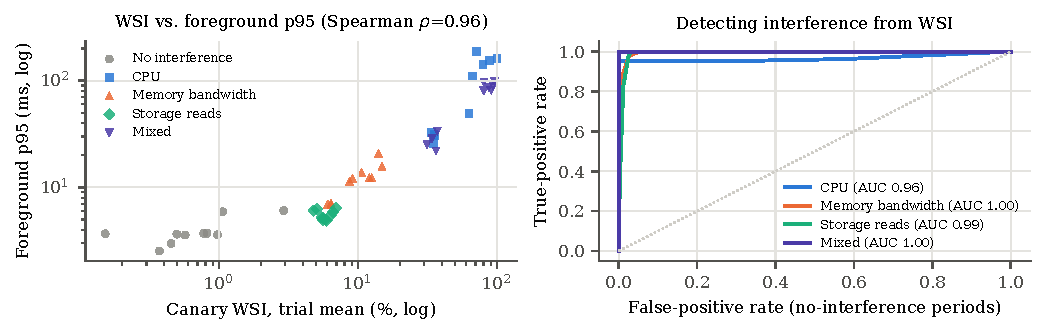
\includegraphics[width=\textwidth]{figures/fig_wsi_validity.pdf}
  \caption{Left: canary WSI against the separate foreground's p95, one point per observe-only trial (log--log). Right: ROC of WSI as an interference detector, per control period.}
  \label{fig:validity}
\end{figure*}

\subsection{Attribution}
In observe-only runs, among control periods whose WSI exceeded the engage threshold, the specificity-ordered rule named the injected resource in 92.4\,\% (CPU), 85.8\,\% (memory bandwidth), and 99.6\,\% (storage) of periods (Table~\ref{tab:attribution}). All 43 misattributed memory-bandwidth periods were labelled CPU, consistent with the scheduling delay that bandwidth-bound workers also cause on a fully subscribed host.

\begin{table}[t]
  \centering
  \caption{Attribution accuracy in observe-only trials.}
  \label{tab:attribution}
  \footnotesize
  \begin{tabular}{lrrr}
\toprule
Workload & Periods $\geq$ engage threshold & Correctly attributed & Accuracy \\
\midrule
CPU & 330 & 305 & 92.4\% \\
Memory bandwidth & 302 & 259 & 85.8\% \\
Storage reads & 281 & 280 & 99.6\% \\
\midrule
No interference & \multicolumn{3}{r}{periods above threshold: 1.2\%} \\
\bottomrule
\end{tabular}
\end{table}

\subsection{Mitigation and its cost}
Table~\ref{tab:main} and Fig.~\ref{fig:tradeoff} compare policies against no mitigation. Under CPU contention, all three mitigations cut median p95 by 87--91\,\%. SmartSwap~v2 (ratio 0.13 [0.03, 0.16]) matched static priority (0.13) and kept 70\,\% of background work, against 51\,\% for v1's unconditional cap. Under mixed interference, all three reached 0.14 at 67\,\% background work. Under storage contention, v1's CPU cap had no effect (1.01), because the workload is I/O-bound. v2 attributed the stall to storage and applied the I/O-priority hint, reducing p95 to 0.52 of the unmitigated value [0.47, 0.75] and to 0.55 of v1's [0.48, 0.71] (raw $p=0.002$, Holm 0.072). That protection cost 76\,\% of background read throughput: Windows' very-low I/O priority throttles aggressively.

Two results are less favourable to v2. First, \textbf{static priority is a strong baseline}. v2 is never significantly better than it on foreground latency (ratios 0.94--1.10, all CIs include 1). Second, under memory-bandwidth contention v2's level-1 priority hint did not bring WSI below the 3\,\% SLO, so v2 escalated to a CPU-rate cap. That cap passed the benefit check (WSI fell by at least 30\,\%) but did not improve the foreground beyond what priority alone achieved (0.60 vs.\ 0.57), and it cost 39\,\% of background work, where static priority kept 98\,\%. The canary was more sensitive to the remaining contention than the foreground was. A benefit check on WSI alone cannot detect this; we return to it in \S\ref{sec:discussion}.

\begin{table*}[t]
  \centering
  \caption{Foreground p95 by workload and policy. Ratio: median over blocks of policy p95 / no-mitigation p95 in the same block, with 95\,\% bootstrap CI. $p_{\mathrm{Holm}}$: exact Wilcoxon, Holm-adjusted over all 37 comparisons. BG kept: background work completed in the foreground window, relative to no mitigation.}
  \label{tab:main}
  \footnotesize
  \begin{tabular}{llrrrr}
\toprule
Workload & Policy & p95 (ms) & p95 ratio vs.\ none [95\% CI] & $p_{\mathrm{Holm}}$ & BG work kept \\
\midrule
No interference & None & 3.95 & -- & -- & 100\% \\
 & Static priority & 3.86 & 0.89 [0.72, 1.00] & 0.469 & -- \\
 & SmartSwap v1 (static cap) & 3.63 & 0.80 [0.56, 1.07] & 1.000 & -- \\
 & SmartSwap v2 (adaptive) & 3.56 & 0.79 [0.56, 0.98] & 0.742 & -- \\
\midrule
CPU & None & 34.92 & -- & -- & 100\% \\
 & Static priority & 4.82 & 0.13 [0.03, 0.17] & 0.072 & 66\% \\
 & SmartSwap v1 (static cap) & 4.18 & 0.09 [0.02, 0.13] & 0.072 & 51\% \\
 & SmartSwap v2 (adaptive) & 4.66 & 0.13 [0.03, 0.16] & 0.072 & 70\% \\
\midrule
Memory bandwidth & None & 10.84 & -- & -- & 100\% \\
 & Static priority & 6.76 & 0.57 [0.44, 0.97] & 0.469 & 98\% \\
 & SmartSwap v1 (static cap) & 6.40 & 0.57 [0.40, 0.79] & 0.105 & 76\% \\
 & SmartSwap v2 (adaptive) & 6.36 & 0.60 [0.43, 0.81] & 0.146 & 61\% \\
\midrule
Storage reads & None & 4.98 & -- & -- & 100\% \\
 & Static priority & 2.91 & 0.58 [0.46, 0.81] & 0.072 & 27\% \\
 & SmartSwap v1 (static cap) & 5.07 & 1.01 [0.96, 1.06] & 1.000 & 101\% \\
 & SmartSwap v2 (adaptive) & 2.68 & 0.52 [0.47, 0.75] & 0.105 & 24\% \\
\midrule
Mixed & None & 29.90 & -- & -- & 100\% \\
 & Static priority & 4.43 & 0.14 [0.08, 0.19] & 0.072 & 67\% \\
 & SmartSwap v1 (static cap) & 4.31 & 0.14 [0.08, 0.19] & 0.072 & 67\% \\
 & SmartSwap v2 (adaptive) & 5.02 & 0.14 [0.09, 0.21] & 0.072 & 67\% \\
\bottomrule
\end{tabular}
\end{table*}

\begin{figure*}[t]
  \centering
  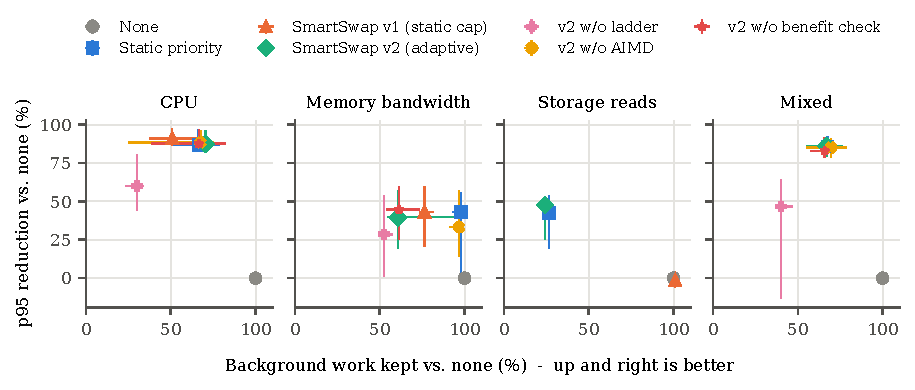
\includegraphics[width=\textwidth]{figures/fig_tradeoff.pdf}
  \caption{Protection versus cost. Each marker is the median over ten blocks; whiskers are 95\,\% bootstrap intervals.}
  \label{fig:tradeoff}
\end{figure*}

\subsection{Ablations}
Removing the ladder, so that the controller goes straight to an AIMD cap, was the only ablation with a large effect. It made p95 $4.8\times$ worse under CPU contention [3.4, 7.0] and $3.8\times$ worse under mixed interference [2.9, 7.9], while keeping only 30--40\,\% of background work (Table~\ref{tab:ablation}). Hard caps duty-cycle the background, and its bursts still collide with the foreground. Removing AIMD (fixed 50\,\% cap) or the benefit check changed p95 by at most 11\,\%, with all intervals including or touching 1. In these stationary workloads the ladder rarely reached level~2 for long, so these two mechanisms had little to act on. The benefit check rolled back ten caps across the study.

\begin{table}[t]
  \centering
  \caption{Ablations: p95 of each variant relative to full v2 in the same block.}
  \label{tab:ablation}
  \footnotesize
  \begin{tabular}{llrrr}
\toprule
Workload & Variant & p95 ratio vs.\ full v2 [95\% CI] & $p_{\mathrm{Holm}}$ & BG work kept \\
\midrule
CPU & v2 w/o ladder & 4.82 [3.38, 7.01] & 0.072 & 30\% \\
 & v2 w/o AIMD & 1.03 [0.95, 1.20] & 1.000 & 67\% \\
 & v2 w/o benefit check & 0.92 [0.83, 1.32] & 1.000 & 67\% \\
Memory bandwidth & v2 w/o ladder & 1.07 [1.00, 1.37] & 0.469 & 53\% \\
 & v2 w/o AIMD & 1.11 [1.00, 1.18] & 0.742 & 97\% \\
 & v2 w/o benefit check & 0.98 [0.89, 1.02] & 1.000 & 61\% \\
Mixed & v2 w/o ladder & 3.84 [2.94, 7.87] & 0.072 & 40\% \\
 & v2 w/o AIMD & 0.97 [0.86, 1.32] & 1.000 & 69\% \\
 & v2 w/o benefit check & 0.97 [0.90, 1.13] & 1.000 & 66\% \\
\bottomrule
\end{tabular}
\end{table}

\subsection{Overhead and verification}
On an idle host, running the canary and controller \emph{lowered} foreground p95 slightly (ratio 0.84 [0.67, 0.97]; p50 0.95). This is consistent with a periodic waker keeping cores out of deep idle states; we report it as an observation, not a benefit. Every one of the 1\,575 actions and 322 reverts in the study matched the kernel state read back after the call.

%%HYBRID%%

%%SLO%%
